\documentclass[11pt,a4paper]{article}
\usepackage{fontspec}
\usepackage{setspace}
\usepackage{amsmath,amsfonts,amssymb,amsthm}
\usepackage[margin=1.1in]{geometry}
\usepackage{graphicx}
\usepackage{subfigure}
\usepackage{listings}
\usepackage{booktabs,dcolumn}                     
\usepackage{fancyhdr}
\usepackage{bbm}
\usepackage{multirow}
\usepackage{booktabs}
\usepackage{harvard}
\usepackage{enumerate}
\newcommand{\ra}[1]{\renewcommand{\arraystretch}{#1}}
\DeclareMathOperator{\tr}{tr}
\DeclareMathOperator{\vect}{vec}
\makeatletter
\newcommand*{\rom}[1]{\expandafter\@slowromancap\romannumeral #1@}
\makeatletter

\setstretch{1.4}
\setlength{\headheight}{15pt} 
\graphicspath{{graphs/}}  

\newtheorem{sectheorem}{Example}

 
\begin{document}
\title{Applied Survival Analysis - January 2016\\Solutions to Lab 3: Comparing survival curves between groups}
\date{\vspace{-5ex}}
\author{\vspace{-5ex}}
\maketitle
\begin{enumerate}[(a)]
\item First, it's better to save our data in a data frame.
\begin{footnotesize}
\begin{verbatim}
> # (a): Artificial data from 2 groups
> surv = c(15,18,19,19,20,16,18,20,23,24)
> fail = c(rep(1,5),c(0,1,0,1,0))
> group = c(rep(0,5),rep(1,5))
> 
> data = data.frame(time = surv, fail = fail, group = group)
\end{verbatim}
\end{footnotesize}
Now we're going to carry out the \emph{Logrank} test using the \verb|survdiff| function of the library \verb|survival|. Please, don't forget to import the library. The syntax of \verb|survdiff| is very similar to the syntax of the survival functions we have come across so far. 
\begin{footnotesize}
\begin{verbatim}
> # Logrank test
> library(survival)
Loading required package: splines
> survdiff( Surv(time,fail) ~ group, data = data)
Call:
survdiff(formula = Surv(time, fail) ~ group, data = data)

        N Observed Expected (O-E)^2/E (O-E)^2/V
group=0 5        5     2.75      1.84         4
group=1 5        2     4.25      1.19         4

 Chisq= 4  on 1 degrees of freedom, p= 0.0455 
\end{verbatim}
\end{footnotesize}
The formula \verb|Surv(time,fail) ~ group| means that we're comparing the survival across the levels of the variable \emph{group}. We can see that the p-value associated with the \emph{Logrank} test is significant. To informally see which group has the survival advantage, we can compare the median survival times between the two groups
\begin{footnotesize}
\begin{verbatim}
> # Compare the median survival between the two groups
> quantile( survfit(Surv(time,fail) ~ group,data = data), probs = 0.5,conf.int = F )
        50
group=0 19
group=1 23
\end{verbatim}
\end{footnotesize}
Since the median survival time is larger in Group1, and after taking into account the p-value of the \emph{Logrank} test, we conclude that 
 Group1 has a significant survival benefit compared to Group0. Note that this analysis was just used to show you the syntax. A proper analysis requires inspection of KM plots along with many other things. \\ 
\textbf{Optional:} Here, we write a \verb|R| function to construct tables that contain the number of failures and the number at risk for each event time.
\begin{footnotesize}
\begin{verbatim}
> # OPTIONAL: function to compute the logrank test
> log.rank = function(surv,fail,group)
+ {
+   # Sort data with respect to time
+   data = data.frame(time = surv,fail = fail,group = group)
+   data = data[order(data$time),]
+   
+   time = data$time
+   delta = data$fail
+   trt = data$group
+   
+   # Distinct event times
+   times.uni = unique(time[delta==1])
+   K = length(times.uni)
+   
+   # Number of failures for each event time
+   dj = table(time[delta == 1])
+   
+   dj.group0 = table(time[delta == 1 & trt == 0])
+   dj.group1 = table(time[delta == 1 & trt == 1])
+   
+   dj.grp0 = rep(0,K)
+   dj.grp0[match(as.numeric(names(dj.group0)),times.uni)] = dj.group0
+   
+   dj.grp1 = dj - dj.grp0
+   
+   # Number at risk for each event time
+   rj = rep(NA,K)
+   rj.grp0 = rep(NA,K)
+   rj.grp1 = rep(NA,K)
+   
+   for (i in 1:K)
+   {
+     rj[i] = sum(time >= times.uni[i])
+     rj.grp0[i] = sum(time[trt==0] >= times.uni[i])
+   }
+   
+   rj.grp1 = rj - rj.grp0
+   
+   out = list()
+   
+   for (i in 1:K)
+   {
+     mat = matrix(nrow = 2,ncol = 2)
+     colnames(mat) = c("Event","No event")
+     rownames(mat) = c("Group0","Group1")
+     
+     mat[1,1] = dj.grp0[i]
+     mat[2,1] = dj.grp1[i]
+     mat[1,2] = rj.grp0[i] - dj.grp0[i]
+     mat[2,2] = rj.grp1[i] - dj.grp1[i]
+     
+     out[[i]] = mat
+   }
+   names(out) = paste("RiskSet",times.uni)
+   
+   out$chi2 = sum(dj.grp0 - rj.grp0*dj/rj)^2/sum( rj.grp0*rj.grp1*dj*(rj-dj)/(rj^2*(rj-1)))
+   
+   return(out)
+ }
> 
> log.rank(data$time,data$fail,data$group)
$`RiskSet 15`
       Event No event
Group0     1        4
Group1     0        5

$`RiskSet 18`
       Event No event
Group0     1        3
Group1     1        3

$`RiskSet 19`
       Event No event
Group0     2        1
Group1     0        3

$`RiskSet 20`
       Event No event
Group0     1        0
Group1     0        3

$`RiskSet 23`
       Event No event
Group0     0        0
Group1     1        1

$chi2
[1] 3.99859
\end{verbatim}
\end{footnotesize}
\item First, we have to import the data into \verb|R|
\begin{footnotesize}
\begin{verbatim}
> # (b): Leukemia Data
> leukem <- read.csv("C:/Applied_Survival_Analysis_Jan2016/lab3/data/leukem.csv")
> leukem[1:4,]
  trt weeks remiss
1   0     1      1
2   0     1      1
3   0     2      1
4   0     2      1
\end{verbatim}
\end{footnotesize}
In \verb|R|, we had better declare a categorical variable as a factor. Factors are extremely important in \verb|R| as some functions work only with them.
 To encode the \emph{trt} variable as a factor, use the following syntax
\begin{footnotesize}
\begin{verbatim}
> # Encode trt as a factor
> leukem$trt[leukem$trt == 1] = "6-MP"
> leukem$trt[leukem$trt == 0] = "Control"
> 
> # Specify the order of the levels
> # so that the control group will be the reference category in regression models
> leukem$trt = factor(leukem$trt,levels = c("Control","6-MP"))
\end{verbatim}
\end{footnotesize}
We used the \verb|levels| option to specify the order of levels of \emph{trt} so that  the control group will be the reference category in a regression model.
\begin{enumerate}[(i)]
\item To tell \verb|R| that we want the KM estimates by treatment group, we just include the \emph{trt} variable in the formula \verb|Surv(weeks,remiss) ~ trt| using the \verb|survfit| function
\begin{footnotesize}
\begin{verbatim}
> # (b)-(i)
> # KM estimates in both groups
> leukem.fit = survfit( Surv(weeks,remiss) ~ trt, data = leukem)
> summary(leukem.fit)
Call: survfit(formula = Surv(weeks, remiss) ~ trt, data = leukem)

                trt=Control 
 time n.risk n.event survival std.err lower 95% CI upper 95% CI
    1     21       2   0.9048  0.0641      0.78754        1.000
    2     19       2   0.8095  0.0857      0.65785        0.996
    3     17       1   0.7619  0.0929      0.59988        0.968
    4     16       2   0.6667  0.1029      0.49268        0.902
    5     14       2   0.5714  0.1080      0.39455        0.828
    8     12       4   0.3810  0.1060      0.22085        0.657
   11      8       2   0.2857  0.0986      0.14529        0.562
   12      6       2   0.1905  0.0857      0.07887        0.460
   15      4       1   0.1429  0.0764      0.05011        0.407
   17      3       1   0.0952  0.0641      0.02549        0.356
   22      2       1   0.0476  0.0465      0.00703        0.322
   23      1       1   0.0000     NaN           NA           NA

                trt=6-MP 
 time n.risk n.event survival std.err lower 95% CI upper 95% CI
    6     21       3    0.857  0.0764        0.720        1.000
    7     17       1    0.807  0.0869        0.653        0.996
   10     15       1    0.753  0.0963        0.586        0.968
   13     12       1    0.690  0.1068        0.510        0.935
   16     11       1    0.627  0.1141        0.439        0.896
   22      7       1    0.538  0.1282        0.337        0.858
   23      6       1    0.448  0.1346        0.249        0.807
\end{verbatim}
\end{footnotesize}
Please, verify that if we specify \verb|levels = c("6-MP","Control")| in the \verb|factor| function above, the treatment group appears first.
\item The \verb|plot| function can take a \verb|survfit| object as an argument. Then, it produces survival curves for each level of the categorical variable which was used in the formula associated with \verb|survfit|. 
\begin{footnotesize}
\begin{verbatim}
> setwd("C:/Applied_Survival_Analysis_Jan2016/lab3/graphs")
> 
> pdf("leukemKM.pdf",height = 6,width = 6)
> plot(leukem.fit, mark.time = F,main = "Comparison of Treatments for Leukemia",
+      ylab = "Survival Probability",
+      xlab = "Time from Remission to Relapse (weeks)",lty = 1:2,col = c("black","red"))
> legend("topright",lty = 1:2,col = c("black","red"),
+        legend = c("Control (N=21)","6-MP (N=21)"),bty = "n")
> dev.off()
\end{verbatim}
\end{footnotesize}
Here, we have to focus on the syntax a little more. The \verb|lty| option defines the line types for each curve in the plot. Note that since we are plotting two survival estimates, \verb|lty| should be a vector of size 2. The first element is associated with the control group while the second one is associated with the treatment group (that's why it's extremely important to know the ordering of the grouping factor!). The same applies to the \verb|col| option, which determines the color of the lines. Through the function \verb|legend| we can add a legend in the graph. The same rules regarding the ordering of the grouping variable apply to the \verb|legend| function. The \verb|bty| option determines the type of box to be drawn around the legend. Please, you're strongly advised to see ?\verb|plot|, ?\verb|plot.survfit| and ?\verb|legend|, and experiment with the above-mentioned rules a little bit.

\begin{figure}[htbp]
	\centering
		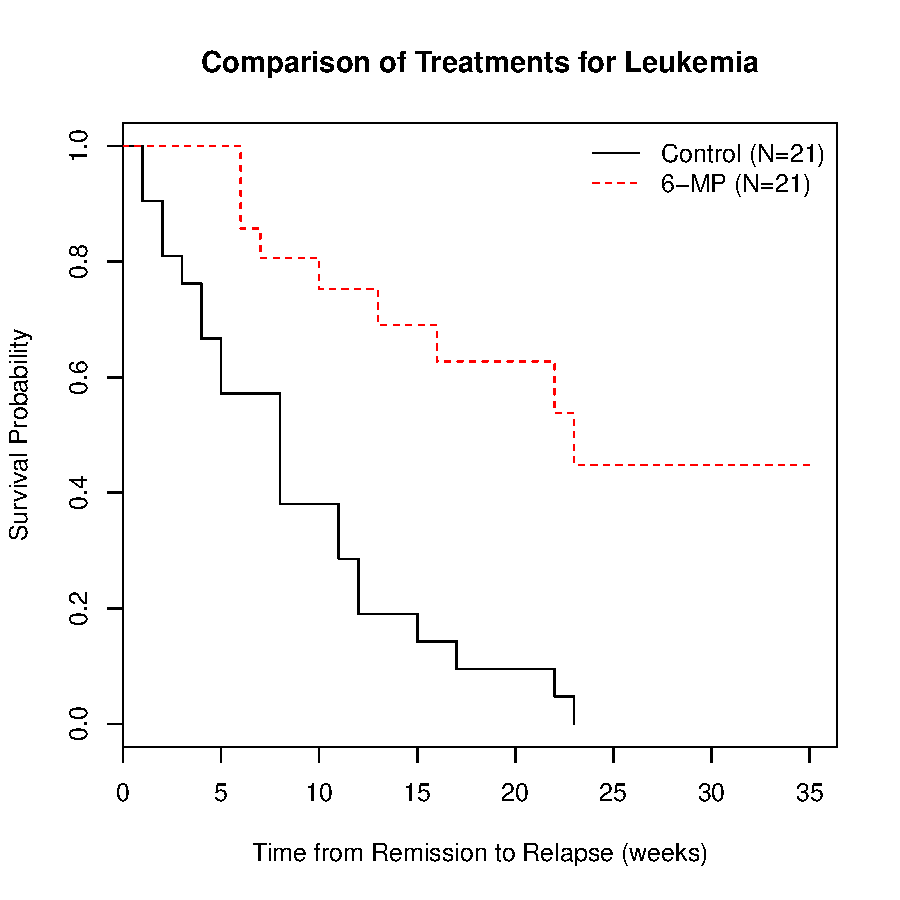
\includegraphics[scale=0.9]{leukemKM.pdf}
		%\rule{35em}{0.5pt}
	\caption{Estimated relapse-free survival for two groups of 42 patients from a leukemia remission study.}
	\label{figure1}
\end{figure}
Turning our attention to the interpretation of the above graph, we can say that the experimental group (6-MP) seems to have a survival benefit compared to the control group. The
relapse free curve is consistently higher in the experimental group than in the control group.
\item The general function in \verb|R| to test for equality of survivor functions is the \verb|survdiff| function. The default test is the \emph{Logrank}, whereas adding the option \verb|rho = 1| you get the \emph{Peto} \& \emph{Peto} modification of the \emph{Gehan-Wilcoxon} test. Please, be aware that this \emph{Wilcoxon} test is slightly \textbf{different} from the one that is available in \verb|STATA| 
An example of both tests
follows:
\begin{footnotesize}
\begin{verbatim}
> # (b)-(iii)
> # Logrank and Wilcoxon tests
> 
> # Logrank - the default
> survdiff(Surv(weeks,remiss) ~ trt, data = leukem)
Call:
survdiff(formula = Surv(weeks, remiss) ~ trt, data = leukem)

             N Observed Expected (O-E)^2/E (O-E)^2/V
trt=Control 21       21     10.7      9.77      16.8
trt=6-MP    21        9     19.3      5.46      16.8

 Chisq= 16.8  on 1 degrees of freedom, p= 4.17e-05 
> 
> # Peto & Peto modification of the Gehan-Wilcoxon test
> survdiff(Surv(weeks,remiss) ~ trt, data = leukem, rho = 1)
Call:
survdiff(formula = Surv(weeks, remiss) ~ trt, data = leukem, 
    rho = 1)

             N Observed Expected (O-E)^2/E (O-E)^2/V
trt=Control 21    14.55     7.68      6.16      14.5
trt=6-MP    21     5.12    12.00      3.94      14.5

 Chisq= 14.5  on 1 degrees of freedom, p= 0.000143 
\end{verbatim}
\end{footnotesize}
In both tests we reject the null hypothesis of equality of the survival curves,
since the p-values are highly significant (p<0.0001  and p=0.0001 and less than
0.05). So we conclude that the survival curves are significantly different
between the treatment groups (in favor of the experimental group). The \emph{Wilcoxon}
test puts more emphasis on early times, and in our case the difference between the
survival estimates in the beginning is not as big as in later times. Thus, the \emph{Wilcoxon}
test statistic is expected to be smaller and its corresponding p-value to be larger (less
significant) than the \emph{Logrank} (p=0.0001 versus p<0.0001). 
\item If we have proportional hazards, then
\begin{align}
\lambda_{2}(t) = \phi\lambda_{1}(t), \ \text{for all}\ t,\nonumber
\end{align}
thus $\Lambda_{2}(t)=\int_{0}^{t}\lambda_{2}(u)du
=\phi\int_{0}^{t}\lambda_{1}(u)du=\phi\Lambda_{1}(t) \Rightarrow$
\begin{align}
\log\Lambda_{2}(t) = \log(\phi) + \log\Lambda_{1}(t).\nonumber
\end{align}
So, the assumption of proportional hazards will be valid if the log cumulative hazards ($\log[-\log S(t)]$ equivalently) are roughly parallel. Thus, applying the \emph{log-log} transformation to the KM estimates we should expect 2 parallel curves. In the \verb|plot| function, just use the option \verb|fun="cloglog"|, which applies the  \emph{log-log} transformation to the KM estimates along with log scale for the x-axis. 
\begin{footnotesize}
\begin{verbatim}
# (b)-(iv)
# Plot of estimated log cumulative hazard
pdf("leukemlogHaz.pdf",height = 6,width = 6)
plot(leukem.fit, mark.time = F,fun="cloglog",
     ylab = "Log cumulative hazard",
     xlab = "Time from Remission to Relapse (weeks)",lty = 1:2,col = c("black","red"))
legend("topleft",lty = 1:2,col = c("black","red"),
       legend = c("Control (N=21)","6-MP (N=21)"),bty = "n")
dev.off()
\end{verbatim}
\end{footnotesize} 
\begin{figure}[htbp]
	\centering
		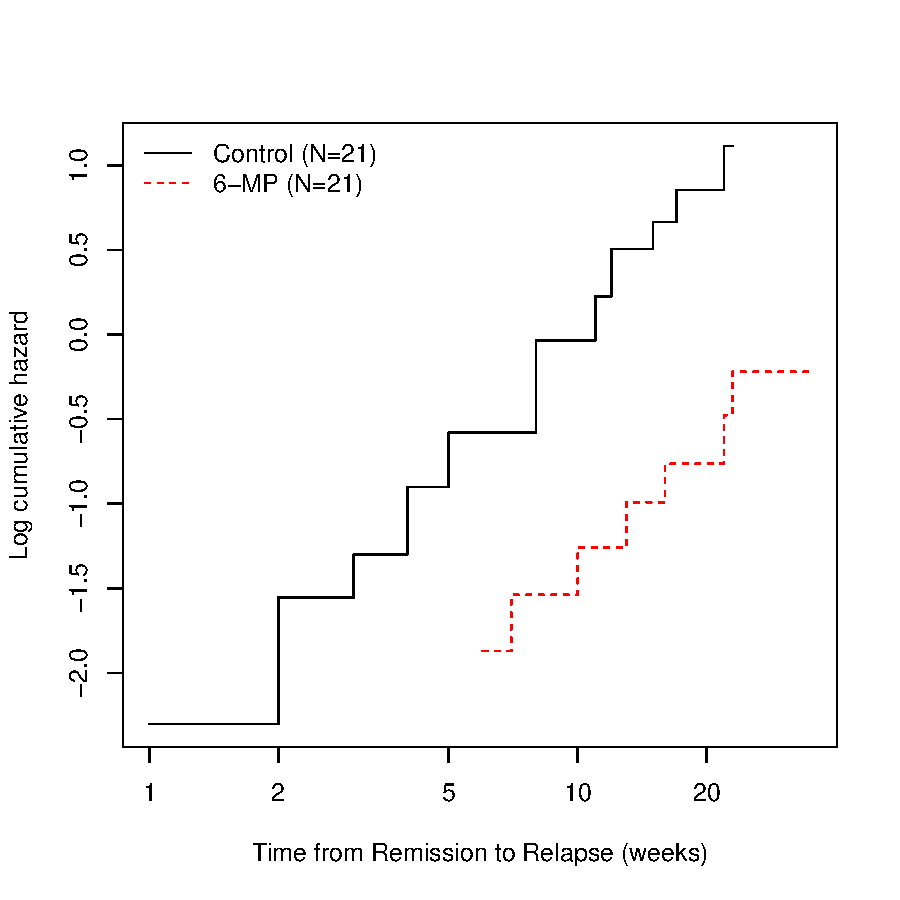
\includegraphics[scale=0.65]{leukemlogHaz.pdf}
		%\rule{35em}{0.5pt}
	\caption{Estimated log cumulative hazards.}
	\label{figure2}
\end{figure}
It seems that the curves are fairly parallel. Thus, we expect the \emph{Logrank} test to be more powerful than the \emph{Wilcoxon} for this scenario, as only the \emph{Logrank} assumes proportional hazards! This is in agreement with the results of part (b)-(iii).
\end{enumerate}
\end{enumerate}



























\end{document}